\chapter{Marco Teórico}

\section{Internet de las Cosas}

La internet de las cosas es un sistema de dispositivos de computación interrelacionados, máquinas mecánicas y digitales, objetos, animales o personas que tienen identificadores únicos y la capacidad de transferir datos a través de una red, sin requerir de interacciones humano a humano o humano a computadora. \\

IoT ha evolucionado desde la convergencia de tecnologías inalámbricas, sistemas micro-electromecánicos, microservicios e internet. La convergencia ha ayudado a derribar las paredes de silos entre la tecnología operativa  y la tecnología de la información, permitiendo que los datos no estructurados generados por máquinas sean analizados para obtener información que impulse mejoras. \cite{TechT2017}\\

Kevin Ashton, cofundador y director ejecutivo del Auto-ID Center de MIT, mencionó por primera vez la internet de las cosas en una presentación que hizo a Procter \& Gamble en 1999. He aquí cómo Ashton explica el potencial de la internet de las cosas:

``Las computadoras de hoy –y, por lo tanto, la internet– dependen casi totalmente de los seres humanos para obtener información. Casi todos los aproximadamente 50 petabytes (un petabyte son 1.024 terabytes) de datos disponibles en internet fueron capturados y creados por seres humanos escribiendo, presionando un botón de grabación, tomando una imagen digital o escaneando un código de barras. \\

El problema es que la gente tiene tiempo, atención y precisión limitados, lo que significa que no son muy buenos para capturar datos sobre cosas en el mundo real. Si tuviéramos computadoras que supieran todo lo que hay que saber acerca de las cosas –utilizando datos que recopilaron sin ninguna ayuda de nosotros– podríamos rastrear y contar todo, y reducir en gran medida los desechos, las pérdidas y el costo. Sabríamos cuándo necesitamos reemplazar, reparar o recordar cosas, y si eran frescas o ya pasadas”. \cite{Asthon2009}\\

\section{Smart House}

El concepto de Smart House implica tres características básicas. En primer lugar, el monitoreo a través de redes de sensores para obtener información sobre la casa y sus residentes. En segundo lugar, los mecanismos que controlan el uso de la comunicación entre dispositivos para permitir la automatización y el acceso remoto. Por último, las interfaces de usuario, como los teléfonos inteligentes y las computadoras que permiten a los usuarios especificar las preferencias, así como presentar información a las personas acerca de estas preferencias. \\

Smart House es un entorno que tiene sistemas sofisticados a través de los cuales se pueden controlar algunas de las cosas de la casa, como luces, puertas, ventanas, además  puede racionalizar el consumo de energía, entre otras funciones mediante el uso de sensores. Básicamente, uno de los beneficios más importantes del uso de la tecnología en las casas, es la prestación de servicios a las personas.\cite{Howedi2016} \\

\section{Hardware}

\subsection{ESP-WROOM-32}

\cite{EW32} Es un potente módulo MCU Wi-Fi + BT + BLE que se dirige a una amplia variedad de aplicaciones, desde redes de sensores de baja potencia hasta las tareas más exigentes, como codificación de voz, transmisión de música y decodificación de MP3.\\

En el núcleo de este módulo está el chip ESP32-D0WDQ6. El chip integrado está diseñado para ser escalable y adaptable. Hay dos núcleos de CPU que se pueden controlar individualmente, y la frecuencia del reloj es ajustable de 80 MHz a 240 MHz. El usuario también puede apagar la CPU y utilizar el coprocesador de baja potencia para monitorear constantemente los periféricos en busca de cambios o cruces de umbrales. ESP32 integra un amplio conjunto de periféricos, que van desde sensores táctiles capacitivos, sensores Hall, interfaz de tarjeta SD, Ethernet, SPI de alta velocidad, UART, I2S e I2C.\\

La integración de Bluetooth, Bluetooth LE y Wi-Fi garantiza que se pueda orientar una amplia gama de aplicaciones, el uso de Wi-Fi permite un gran alcance físico y conexión directa a Internet a través de Wi-Fi, mientras usa Bluetooth, le permite al usuario conectarse convenientemente al teléfono o transmitir balizas de baja energía para su detección. La corriente de reposo del chip ESP32 es inferior a 5 uA, lo que lo hace adecuado para aplicaciones de electrónica con batería y portátiles. ESP32 admite una velocidad de datos de hasta 150 Mbps y una potencia de salida de 20.5 dBm en la antena para garantizar el rango físico más amplio.\\

El sistema operativo elegido para ESP32 es freeRTOS con LwIP; TLS 1.2 con aceleración de hardware está integrado también. También se admite la actualización segura (cifrada) a través del aire (OTA), de modo que los desarrolladores puedan actualizar continuamente sus productos incluso después de su lanzamiento. \\


\begin{figure}
	\centering
	\caption{ESP WROOM 32}
	\label{fig:esp32-wroom-s32-00}
	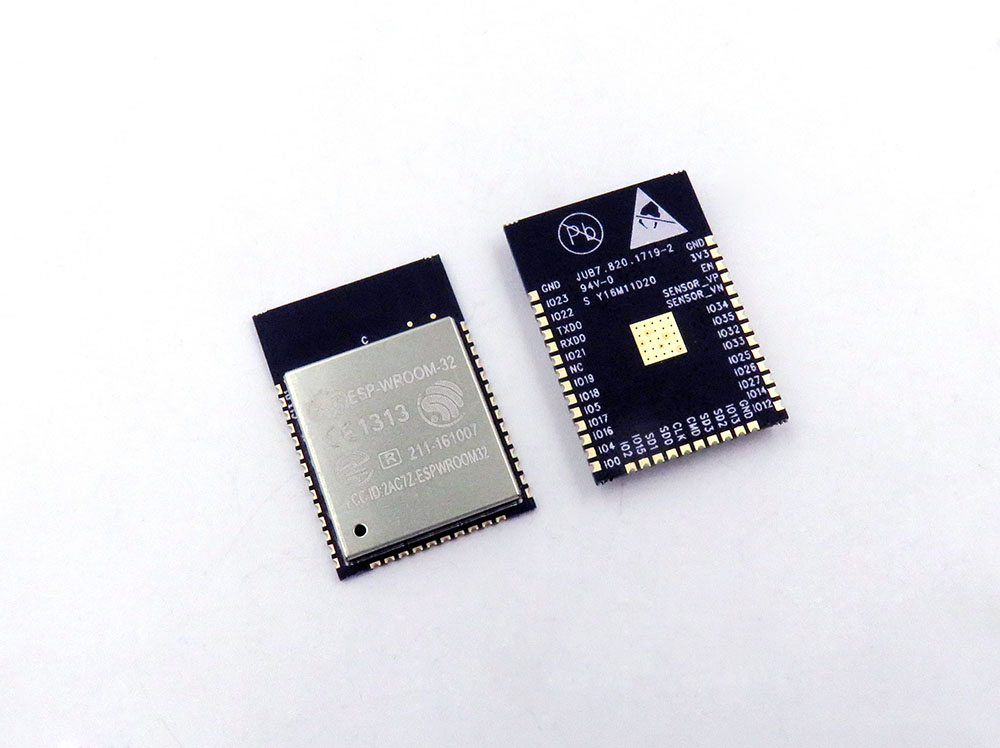
\includegraphics{Imagenes/esp32-wroom-s32-00}
\end{figure}

%http://www.electrodragon.com/product/wroom-32/


\subsection{Control de potencia AC por ángulo de fase}

%TRIACS, detector de cruce por cero, optoacopladores

\subsection{Switch con transistores}

%Switch y control de cargas DC

\subsection{I2C}

\subsection{Optoacoplador}

\subsection{Sensores}

\subsubsection{Luminosidad}

\subsection{Cargas AC}

\subsection{Cargas DC}

\section{Software}

\subsection{RTOS}

\cite{SO} Los sistemas operativos en tiempo real, tienen como parámetro clave al tiempo, ya que en gran variedad de situaciones, como por ejemplo, un proceso industrial, se requiere recolectar múltiples datos, los cuales son usados para el control de múltiples procesos, los cuales deben ser ejecutados en determinados instantes, de no ser así, podría causar desde la mala ejecución de una tarea, hasta un accidente según la delicadeza del proceso.\\ 


Para procesos con nula tolerancia a fallos, se conoce como un sistema en tiempo real duro, muchos de estos sistemas se encuentran en el control de procesos industriales, en aeronáutica, en la milicia y en áreas de aplicación similares. el caso contrario, cuando se tiene cierta tolerancia a que muy ocasionalmente existan fallos, se conoce como sistema en tiempo real suave, los sistemas de audio digital o de multimedia están en esta categoría. Los teléfonos digitales también son ejemplos de sistema en tiempo real suave. \\


%Otro tipo de sistema operativo es el sistema en tiempo real. Estos sistemas se caracterizan por tener el tiempo como un parámetro clave. Por ejemplo, en los sistemas de control de procesos industriales, las computadoras en tiempo real tienen que recolectar datos acerca del proceso de producción y utilizarlos para controlar las máquinas en la fábrica. A menudo hay tiempos de entrega estrictos que se deben cumplir. Por ejemplo, si un auto se desplaza sobre una línea de ensamblaje, deben lle- varse a cabo ciertas acciones en determinados instantes. Si un robot soldador realiza su trabajo de soldadura antes o después de tiempo, el auto se arruinará. Si la acción debe ocurrir sin excepción en cierto momento (o dentro de cierto rango), tenemos un sistema en tiempo real duro. Muchos de estos sistemas se encuentran en el control de procesos industriales, en aeronáutica, en la milicia y en áreas de aplicación similares. Estos sistemas deben proveer garantías absolutas de que cierta acción ocurrirá en un instante determinado. 

%Otro tipo de sistema en tiempo real es el sistema en tiempo real suave, en el cual es acepta- ble que muy ocasionalmente se pueda fallar a un tiempo predeterminado. Los sistemas de audio di- gital o de multimedia están en esta categoría. Los teléfonos digitales también son ejemplos de sistema en tiempo real suave. 

``Como en los sistemas en tiempo real es crucial cumplir con tiempos predeterminados para realizar una acción, algunas veces el sistema operativo es simplemente una biblioteca enlazada con los programas de aplicación, en donde todo está acoplado en forma estrecha y no hay protección entre cada una de las partes del sistema. Un ejemplo de este tipo de sistema en tiempo real es freeRTOS.  Las categorías de sistemas para computadoras de bolsillo, sistemas integrados y sistemas en tiempo real se traslapan en forma considerable. Casi todos ellos tienen por lo menos ciertos aspectos de tiempo real suave. Los sistemas integrados y de tiempo real sólo ejecutan software que colocan los diseñadores del sistema; los usuarios no pueden agregar su propio software, lo cual facilita la protección. \\

Los sistemas de computadoras de bolsillo y los sistemas integrados están diseñados para los consumidores, mientras que los sistemas en tiempo real son más adecuados para el uso industrial. Sin embargo, tienen ciertas características en común''.\\

\subsection{ESP-IDF}

ESP-IDF es el entorno de desarrollo oficial para el ESP32 desarrollado por Espressif System, el cual mediante una serie de comandos específicos escritos en la terminal (para el caso de linux), permite realizar una configuración del ESP32 en cuanto a su funcionamiento, es decir, permite encender o apagar características como el WiFi, el Bluetooth o realizar particiones de memoria, ademas de esto, se puede cargar el código por el puerto USB al ESP32, al igual que se puede visualizar la información generada por el ESP32 por este mismo puerto.\\

\subsubsection{Particiones}
\subsubsection{Consola}
\subsubsection{OTA}
\subsubsection{HTTP Request}
\subsubsection{Timers}

\subsection{Heroku}

\subsection{Framework IoT}
%Framework del profesor Cesar Alvarez

\subsection{HTTP}

\subsection{JSON}

\subsection{Proteus}
